\documentclass{standalone}
\usepackage{circuitikz}
\usepackage{schemabloc}

\begin{document}
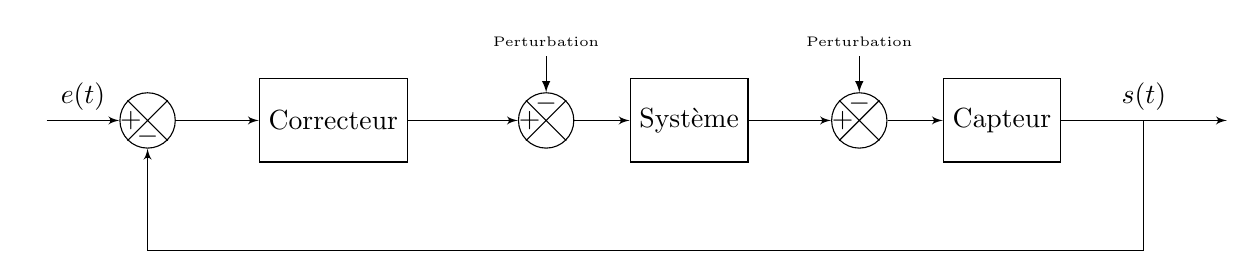
\begin{tikzpicture}
\sbEntree{E}
\sbComp{comp}{E}
\sbRelier[$e(t)$]{E}{comp}
\sbBloc[3]{B1}{Correcteur}{comp}
\sbRelier{comp}{B1}
\sbComph[5]{comp1}{B1}
\sbRelier{B1}{comp1}
\sbBloc{B2}{Système}{comp1}
\sbRelier{comp1}{B2}
\sbComph{comp2}{B2}
\sbRelier{B2}{comp2}
\sbBloc{B3}{Capteur}{comp2}
\sbRelier{comp2}{B3}
\sbSortie[6]{S}{B3}
\sbRelier[$s(t)$]{B3}{S}
\sbRenvoi{B3-S}{comp}{}
\node[above of=comp1](comp1a) {\tiny Perturbation};
\node[above of=comp2](comp2a) {\tiny Perturbation};
\draw[->,>=latex] (comp1a) -- (comp1);
\draw[->,>=latex] (comp2a) -- (comp2);
\end{tikzpicture}
\end{document}